\documentclass[11pt]{article}
%Gummi|063|=)
\usepackage{datetime}
\usepackage{mathtools}
\usepackage{listings}
\usepackage{graphicx}
\title{\textbf{Simulating Kerr Geodesics}}
\author{Ian Smith}
\date{June 2015}
\graphicspath{ {images/} }
\begin{document}

\maketitle

\abstract
A simple and accurate numerical method is presented aimed at generating 4D geodesics for particles and photons in the Kerr spacetime.  Particular attention is paid to the problem of generating a variety of usable initial conditions for the simulator.  Sources of error are quantified and monitored as a matter of course.  The source code for the suite of programs is publically available under a BSD licence.

\section{Bound Orbits in the Kerr Spacetime}

The starting point is the Kerr line element expressed in terms of the commonly used Boyer-Lindquist coordinates.

\begin{align*}
d s^2 &= \frac{ \sin^2 \theta } {r^2 + a^2 \cos^2 \theta} (a dt - (r^2 + a^2)d \phi )^2 + \frac{ r^2 + a^2 \cos^2 \theta } {(r^2 - 2Mr  + a^2)} d r^2 \\
&+ (r^2 + a^2 \cos^2 \theta) d \theta^2 + \frac{ (r^2 - 2Mr  + a^2) } {r^2 + a^2 \cos^2 \theta} (dt - a \sin^2 \theta d \phi )^2
\end{align*}

The geodesic equations for the Kerr spacetime are complex second order differential equations which are well known and can be solved using standard numerical integration techniques, typically one of the Runge-Kutta methods.  Unfortunately this approach is unsuitable for studying horizon crossing scenarios because in these cases the $t$ variable becomes "unresponsive" near the outer horizon and slows the simulation to a near standstill without ever getting there.

Rather than attempting to formulate and solve these geodesic equations directly, the approach taken here is to evolve the first order equations of motion expressed in terms of the constants of motion $E$ (energy), $L$ (equatorial angular momentum), and $Q$ (Carter's constant).  Because $t$ is not an integration variable here, these equations do not grind to a halt at the horizon.

The approach is so straightforward that the complete simulator script consists of just over a hundred lines of Python code \cite{m4r35n357}.

\subsection {Equations of motion}

This is the well known set of equations describing Kerr orbits in terms of $E$, $L$, and $Q$:
\begin{align}
\frac{d t}{d \lambda} &= \frac{(r^2 + a^2) \left((r^2 + a^2) E - aL \right)} {(r^2 - 2Mr  + a^2)} + a(L - aE \sin^2 \theta) \\
\frac{d r}{d \lambda} &= \pm \sqrt {R(r)} \\
\frac{d \theta}{d \lambda} &= \pm \sqrt {\Theta (\theta)} \\
\frac{d \phi}{d \lambda} &= \frac{a \left((r^2 + a^2) E - aL \right)} {(r^2 - 2Mr  + a^2)} + \left(\frac {L} {\sin^2 \theta} -aE \right)
\end{align}
where
\begin{equation}
d \lambda = \frac {d \tau} {(r^2 + a^2 \cos^2\theta)}
\end{equation}
These are essentially equations 2 and 3 from \cite{wilkins}, fully expanded except for the two potential functions $R$ and $\Theta$ which, together with their differentials, are defined in equations 6-9 below.

Notice also the use of the "Carter-Mino" time variable, $\lambda$, to render the $R$ and $\Theta$ equations (plus their differentials of course) mutually independent.  In terms of this time variable, the potentials are simply the squares of the $r$ and $\theta$ velocities.

\begin{align}
R(r) &= \left((r^2 + a^2) E - aL \right)^2 - (r^2 - 2Mr  + a^2) \left(Q + ( L - aE)^2 + \mu^2 r^2 \right) \\
\frac{d R(r)}{d r} &= 4rE \left((r^2 + a^2)E - aL \right) - (2r - 2M) \left(Q + ( L - aE)^2 + \mu^2 r^2 \right) - 2\mu^2r(r^2 - 2Mr  + a^2) \\
\Theta (\theta) &= Q - {\cos^2 \theta } \left( \frac{L^2}{\sin^2 \theta } + a^2( \mu^2 - E^2) \right) \\
\frac{d \Theta (\theta)}{d \theta} &= 2 \cos \theta \sin \theta \left(\frac{L^2} {\sin^2 \theta } + a^2(\mu^2 - E^2) \right) +\frac{2 L^2 \cos^3 \theta } {\sin^3 \theta }
\end{align}

The $t$ and $\phi$ equations (1 and 4) can be evolved trivially using the Euler method, but the $R$ and $\Theta$ equations (2 and 3) require a little more effort.  Because of the square roots the Euler approach is severely hampered by the need to identify turning points, which is difficult to achieve reliably, and even harder to do without compromising the accuracy of the simulation.  The approach described here is to use a symplectic Stormer-Verlet integrator \cite{hairer} to evolve the $R$ and $\Theta$ equations, which turns out to be a surprisingly simple solution, and is possible because the potential equations (when squared) are both of the form:

\begin{equation}
\dot x^2 - V(x) = 0
\end{equation}

This expresison is used to quantify the integration errors, whilst the two differentiated potentials in equations 7 and 9 are used for velocity updates in the integrator routines.

The simulator uses composition \cite{hairer} to step the (even) integration order from 2 in the case of basic Stormer-Verlet, up to a maximum of 10th order.

\section{Finding initial conditions}

Another difficulty in generating orbits is the problem of generating initial conditions.  Finding an interesting set by trial and error is hard, partly because many combinations of the constants of motion are unphysical.

Here I present a straightforward way of generating two types of bound orbits in three spatial dimensions.  It is based on solving sets of three potential equations under various conditions using the three constants of motion $E$, $L$, and $Q$ as variables, and turning points of the potentials as constant parameters.

\subsection{Constant radius ("spherical") orbits}

For constant radius orbits at $r_0$, we are looking for a double root (local maximum) of the quartic $R(r)$, in other words we want the radial velocity to be zero, and its differential to also be zero so that the radial speed remains zero during the orbit.  $\Theta (\theta)$ will also be zero at the maximum deviation from equatorial (the minimum value of $\theta$).

\begin{align}
R(r_0, E, L, Q) &= 0 \\
\frac{d R(r_0, E, L, Q)}{d r} &= 0 \\
\Theta(\theta_{MIN}, E, L, Q) &= 0
\end{align}

\subsection{Variable radius ("spherical shell") orbits}

For variable radius orbits we are looking for two distinct roots of the quartic $R(r)$, in other words that the orbit is bound between two $r$ values, $r_1$ and $r_2$.  The $\Theta (\theta)$ condition is unchanged from the constant radius case above.

\begin{align}
R(r_1, E, L, Q) &= 0 \\
R(r_2, E, L, Q) &= 0 \\
\Theta(\theta_{MIN}, E, L, Q) &= 0
\end{align}

\subsection{Plummeting (an aside)}

These "orbits" are not the focus of this article, but are easily specified by setting $L = 0$ after generating a spherical orbit as in equations 11-13 above.

\subsection{Finding the roots}

Equations 11-13 and 14-16 can of course be solved by various root-finding techniques, but the equations and algorithms can often become messy and potentially error-prone, with no easy way to check intermediate results.  For this work I took a simpler approach; forming a sum-of-squares error function from the constraints described above, minimizing it, then making sure it is sufficiently close to zero.  By experience I have found that the Nelder-Mead algorithm from Scipy converges reliably from zero initial conditions on $E$, $L$, and $Q$, and so far have found no reason to look elsewhere.

A typical invocation of tthe suite of progrms might be:
\begin{verbatim}
./genparam.py 3.0 12.0 0.3 1.0 1.0 >test 2>potential; ./rungraphics test
\end{verbatim}
which generates an orbit bound between 3 and 12 radial units and with a minimum latitude of 0.3 radians (starting from the "north pole" of course).
Once the optimization has terminated the generation script then writes an initial conditions file (including the final values of $E$, $L$, and $Q$ as well as optimizer status) in JSON format for use as input to the simulator.  Here is an example:
\begin{verbatim}
{ "M" : 1.0,
  "a" : 1.0,
  "mu" : 1.0,
  "E" : 0.937868402897,
  "Lz" : 2.16351904692,
  "C" : 2.51243192834,
  "r" : 7.5,
  "theta" : 1.57079632679,
  "time" : 20.0,
  "step" : 0.001,
  "integratorOrder" : 2,
  "error" : 3.106239408e-24,
  "success" : "True",
  "message" : "Optimization terminated successfully."
}
\end{verbatim}
The simulator takes this input, calculates the geodesic and writes its output data in JSON format (for the default timestep the output file is approximately 6.7MB).  A static image of the corresponding geodesic is shown below.  VPython allows the user to zoom and rotate the view, and watch it evolve.
\begin{figure}[h]
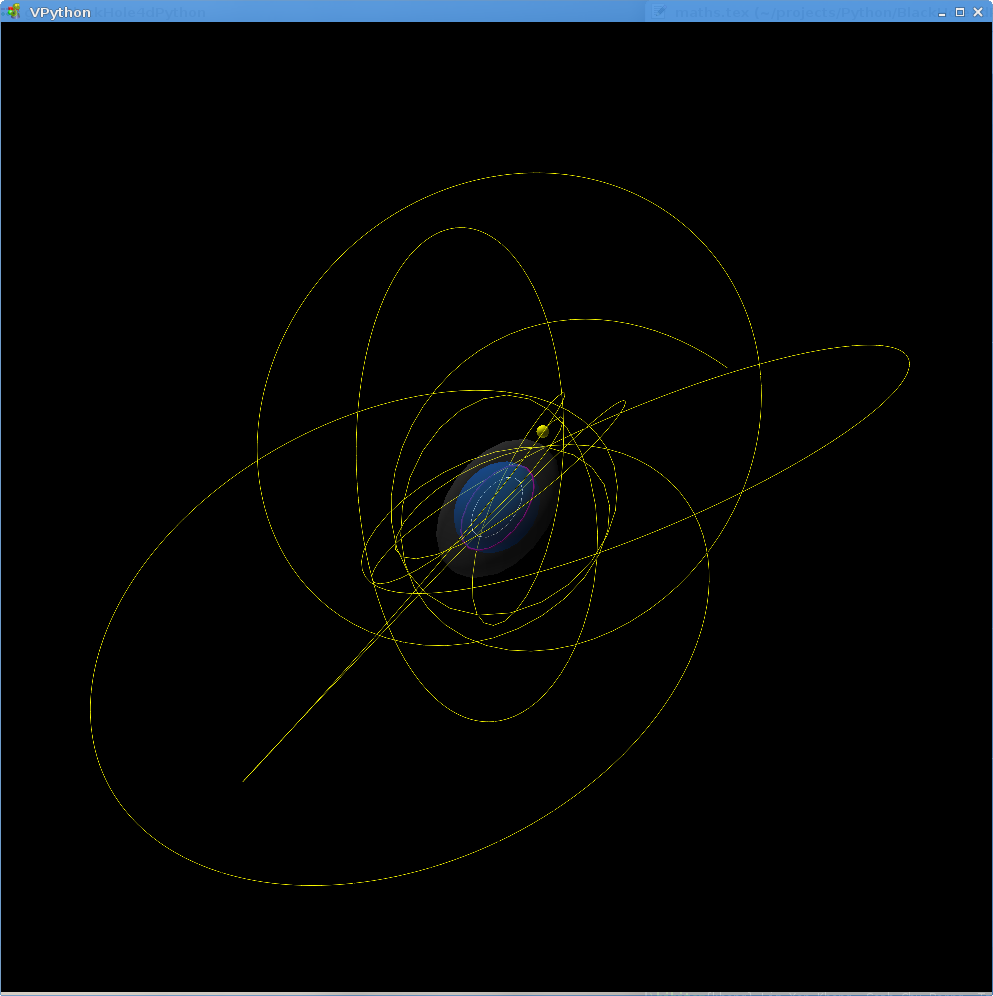
\includegraphics[width=\textwidth]{Screenshot}
\end{figure}
The output of the simulator has been informally checked against a number of publically available result sets and programs to guard against the possibility of gross errors.  This includes  but is not limited to the program GRorbits for equatorial geodesics \cite{grorbits}, together with published papers for spherical particle orbits \cite{teo}, and photon orbits \cite{kheng}.

\subsection{. . . but are they REALLY geodesics?}

Despite the high level of accuracy which the symplectic integrator can achieve for $r$ and $\theta$, this provides no guarantee that the complete solution is an accurate geodesic.  To verify this, we can evaluate the four-velocity norm of the path by plugging all the coordinate derivatives into the line element.  This error data is part of the JSON output of the simulation.  The figure below shows the errors in the simulation: blue is the radial error, red the latitudinal, and green the (deviation from) four-velocity norm, all plotted against a false dB scale (where 0dB = 1.0).
\begin{figure}[h]
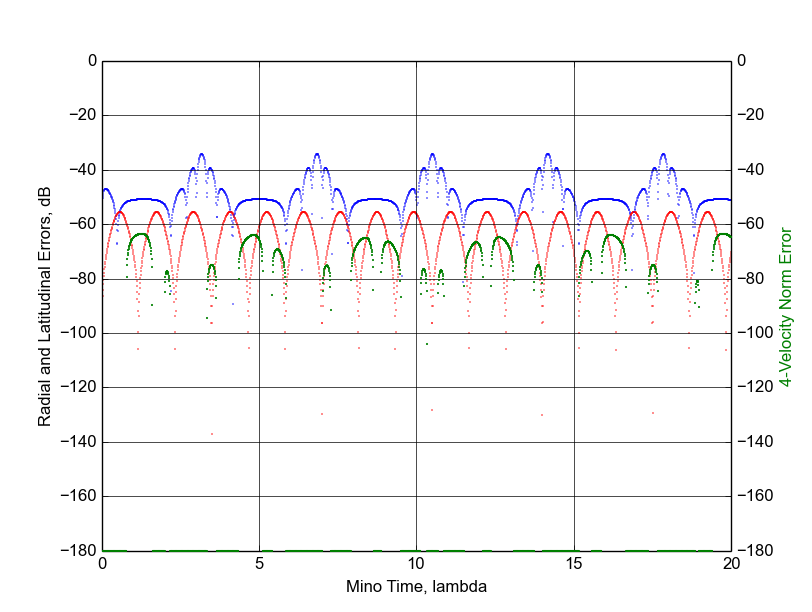
\includegraphics[width=\textwidth]{figure_1}
\end{figure}
This type of error plot makes it easy to see the effects on accuracy of changing the timestep and integrator order; the default values of 2nd order integration and a fairly course timestep are intended to encourage experimentation.

\section{The programs}

The sources for the programs \cite{m4r35n357} described here are publically available on GitHub, under a BSD licence.  These are part of a suite of very small scripts and programs which are intended to implement the methods in this article as concisely as possible.  There is a short README file in the root directory which gives basic instructions for running the simulations.

\begin{thebibliography}{1}
\bibitem{wilkins} Wilkins, D.C., "Bound Geodesics in the Kerr Metric"
\bibitem{hairer}  Hairer, E., Hairer, M., "GniCodes - Matlab programs for geometric numerical integration "
\bibitem{kheng} Lim Yen Kheng, Seah Chu Perng, Tan Boon Sze Jackson, "Massive Particle Orbits Around Kerr Black Holes"
\bibitem{teo} Teo, E, "Spherical photon orbits around a Kerr black hole"
\bibitem{grorbits} Tujela, S., "GRorbits, http://stuleja.org/grorbits/"
\bibitem{m4r35n357} Smith, I. C., "4D Kerr Spacetime Geodesic calculation and display, https://github.com/m4r35n357/BlackHole4DPython.git"
\end{thebibliography}

\end{document}

